% ============================================================================
%  Figure 2 — Pipeline figure (Step 1 / Step 6 of paper-writing workflow)
%  ----------------------------------------------------------------------------
%  Five-panel pipeline. Panel C (TCO + MC interior sampling) is the visual
%  centerpiece — this is the structural difference vs Wollschläger et al. 2025.
%
%  Required packages in the main .tex preamble:
%     \usepackage{tikz}
%     \usetikzlibrary{positioning, arrows.meta, fit, shapes.geometric, calc}
%     \usepackage{xcolor}
% ============================================================================

\begin{figure*}[t]
\centering
% \definecolor{truecolor}{HTML}{2E7D32}     % factual green
% \definecolor{falsecolor}{HTML}{C62828}    % factual red
% \definecolor{retaincolor}{HTML}{616161}   % neutral gray
% \definecolor{methodcolor}{HTML}{1565C0}   % method blue
% \definecolor{conecolor}{HTML}{1565C0!25}  % translucent cone fill
% \definecolor{accentcolor}{HTML}{C62828}   % red callout for l*


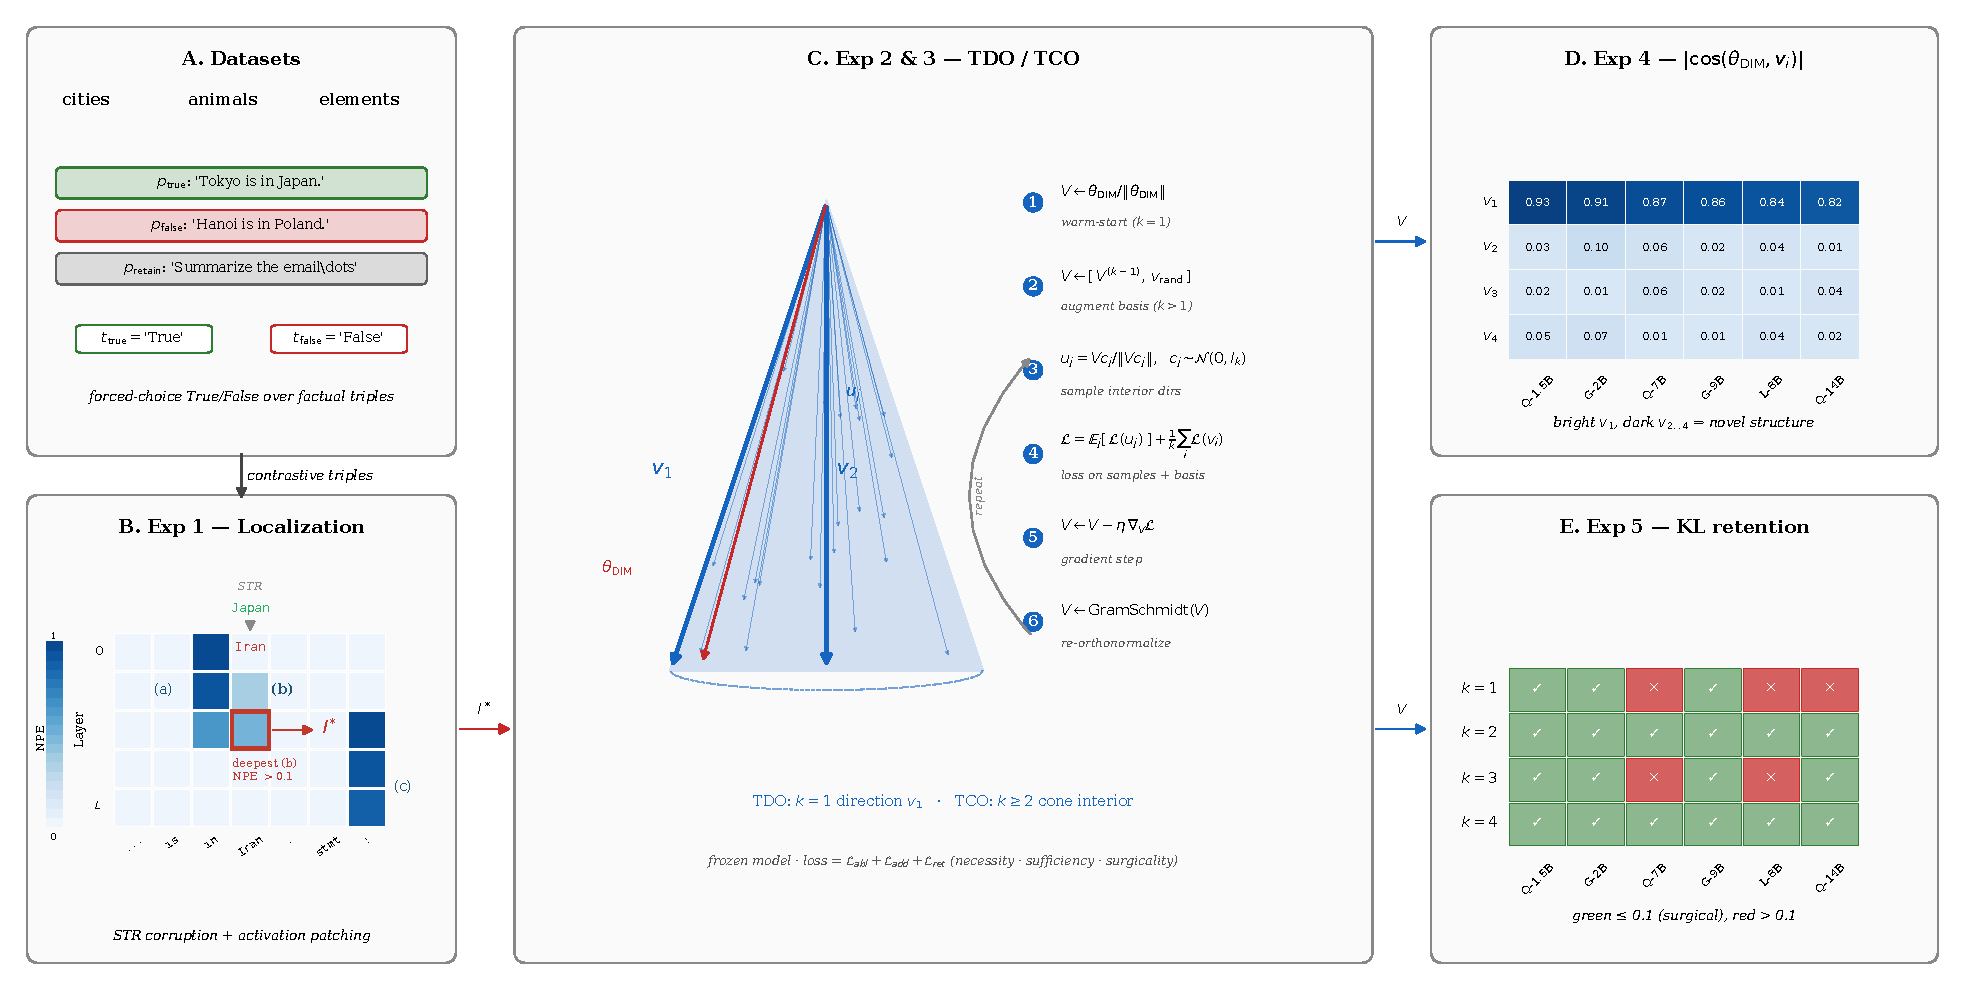
\includegraphics[width=\linewidth]{figures/fig_pipeline.pdf}

% \begin{tikzpicture}[
%     >={Stealth[length=2.2mm]},
%     box/.style   = {draw, rounded corners=2pt, inner sep=4pt, align=center},
%     panel/.style = {draw, rounded corners=3pt, inner sep=6pt, align=center,
%                     fill=gray!3, line width=0.6pt},
%     arr/.style   = {-{Stealth[length=2mm]}, line width=0.7pt},
%     label/.style = {font=\scriptsize\itshape}
% ]

% % ===========================================================================
% % PANEL A — DATASETS (left, ~22% width)
% % ===========================================================================
% \node[panel, minimum width=3.4cm, minimum height=4.6cm] (A) at (0,0) {};
% \node[anchor=north, font=\small\bfseries] at (A.north) {A. Datasets};

% % Three domain icons row
% \node[font=\scriptsize] at ($(A.north) + (-0.95,-0.55)$) {\bfseries cities};
% \node[font=\scriptsize] at ($(A.north) + ( 0.00,-0.55)$) {\bfseries animals};
% \node[font=\scriptsize] at ($(A.north) + ( 0.95,-0.55)$) {\bfseries elements};

% % Forced-choice triple, shown as colored bars (T/F/R)
% \node[box, fill=truecolor!18, draw=truecolor!60, minimum width=2.9cm,
%       minimum height=0.32cm, font=\tiny] (ptrue) at ($(A.center) + (0,0.4)$)
%       {$p_{\text{true}}$: ``Tokyo is in Japan.''};
% \node[box, fill=falsecolor!18, draw=falsecolor!60, minimum width=2.9cm,
%       minimum height=0.32cm, font=\tiny, below=1mm of ptrue] (pfalse)
%       {$p_{\text{false}}$: ``Hanoi is in Poland.''};
% \node[box, fill=retaincolor!15, draw=retaincolor!60, minimum width=2.9cm,
%       minimum height=0.32cm, font=\tiny, below=1mm of pfalse] (pretain)
%       {$p_{\text{retain}}$: ``Summarize the email\dots''};

% % Targets
% \node[box, draw=truecolor, minimum width=0.85cm, minimum height=0.32cm,
%       font=\tiny] (ttrue) at ($(pretain.south) + (-0.75,-0.45)$)
%       {$t_{\text{true}}{=}$``True''};
% \node[box, draw=falsecolor, minimum width=0.85cm, minimum height=0.32cm,
%       font=\tiny] (tfalse) at ($(pretain.south) + ( 0.75,-0.45)$)
%       {$t_{\text{false}}{=}$``False''};

% % Differentiator caption
% \node[font=\tiny\itshape, text width=3.2cm, align=center] at
%       ($(A.south) + (0,0.25)$) {forced-choice True/False over factual triples};

% % ===========================================================================
% % PANEL B — LOCALIZATION (top center-left, ~22% width)
% % ===========================================================================
% \node[panel, right=0.8cm of A, minimum width=3.4cm, minimum height=4.6cm,
%       yshift=1.3cm] (B) {};
% \node[anchor=north, font=\small\bfseries] at (B.north)
%      {B. Exp~1 — Localization};

% % Transformer column (schematic)
% \foreach \i/\y in {7/2.4, 6/2.0, 5/1.6, 4/1.2, 3/0.8, 2/0.4, 1/0.0} {
%   \draw[fill=methodcolor!15, draw=methodcolor!60, rounded corners=1pt]
%       ($(B.west) + (0.45, \y - 1.3)$) rectangle
%       ($(B.west) + (1.05, \y - 1.0)$);
% }
% % l* highlight (one of the middle blocks)
% \draw[fill=accentcolor!25, draw=accentcolor, line width=0.8pt, rounded corners=1pt]
%     ($(B.west) + (0.45, 0.4 - 1.3)$) rectangle
%     ($(B.west) + (1.05, 0.4 - 1.0)$);
% \node[font=\tiny, anchor=east, text=accentcolor]
%     at ($(B.west) + (0.42, 0.55 - 1.3)$) {$l^{*}$};

% % NPE mini-heatmap to the right of the column
% \foreach \i in {0,1,2,3,4} {
%   \foreach \j in {0,1,2,3,4,5,6} {
%     \pgfmathsetmacro{\val}{abs(sin((\i+\j)*20)) * 80}
%     \fill[methodcolor!\val] ($(B.west) + (1.35 + 0.18*\i, -1.3 + 0.21*\j)$)
%         rectangle ++(0.16,0.18);
%   }
% }
% % Group annotations
% \node[font=\tiny] at ($(B.west) + (2.5, -0.95)$) {(a)};
% \node[font=\tiny] at ($(B.west) + (2.5,  0.05)$) {(b)};
% \node[font=\tiny] at ($(B.west) + (2.5,  1.05)$) {(c)};

% \node[font=\tiny\itshape, text width=3.0cm, align=center]
%     at ($(B.south) + (0,0.25)$)
%     {STR corruption + denoising patch sweep};

% % Arrow from A to B
% \draw[arr] (A.east) -- node[above, label, pos=0.5]{contrastive triples}
%             (B.west |- A.east);
% % Arrow from B output to Panel C
% \draw[arr] (B.south) -- ++(0,-0.4)
%     node[right, label, pos=0.5]{\,\,$l^{*}$};

% % ===========================================================================
% % PANEL C — TCO with MC INTERIOR SAMPLING  (center, ~38% width — CENTERPIECE)
% % ===========================================================================
% \node[panel, right=0.8cm of B, minimum width=6.6cm, minimum height=6.0cm,
%       yshift=-0.65cm, fill=methodcolor!2] (C) {};
% \node[anchor=north, font=\small\bfseries] at (C.north)
%      {C. Exp~2 \& 3 — TDO / TCO with Monte-Carlo interior sampling};

% % Cone shape (translucent triangle as 2D sketch of a cone)
% \coordinate (apex) at ($(C.center) + (0,1.2)$);
% \coordinate (baseL) at ($(C.center) + (-1.6,-1.5)$);
% \coordinate (baseR) at ($(C.center) + ( 1.6,-1.5)$);
% \fill[conecolor] (apex) -- (baseL) -- (baseR) -- cycle;
% \draw[methodcolor, line width=0.6pt] (apex) -- (baseL);
% \draw[methodcolor, line width=0.6pt] (apex) -- (baseR);
% \draw[methodcolor!60, dashed, line width=0.4pt] (baseL) -- (baseR);

% % Cone elliptical base (perspective hint)
% \draw[methodcolor!60, dashed, line width=0.4pt]
%     (baseL) .. controls ($(C.center) + (-0.5,-1.7)$) and
%                        ($(C.center) + ( 0.5,-1.7)$) ..
%     (baseR);

% % Two basis vectors v1, v2 (bold arrows along cone edges)
% \draw[->, methodcolor, line width=1.1pt] (apex) -- (baseL)
%     node[pos=0.6, left=1pt, font=\scriptsize] {$v_1$};
% \draw[->, methodcolor, line width=1.1pt] (apex) --
%     ($(C.center) + (0.0,-1.5)$)
%     node[pos=0.7, left=1pt, font=\scriptsize] {$v_2$};

% % DIM vector (thin red, nearly aligned with v1, slightly off)
% \draw[->, accentcolor, line width=0.6pt] (apex) -- ($(baseL) + (0.25,0.05)$)
%     node[pos=0.55, right=1pt, font=\scriptsize\itshape] {$\theta_{\text{DIM}}$};

% % Interior MC samples (~25 thin gray arrows from apex into cone)
% \foreach \t in {-1.4,-1.2,-1.0,-0.8,-0.6,-0.4,-0.2,0,0.2,0.4,0.6,0.8,1.0,1.2,1.4} {
%   \pgfmathsetmacro{\dx}{\t * 1.0}
%   \pgfmathsetmacro{\dy}{-1.3 + 0.15*abs(\t)}
%   \draw[->, methodcolor!55, line width=0.25pt]
%       (apex) -- ($(apex) + (\dx, \dy)$);
% }
% \foreach \t in {-1.1,-0.7,-0.3,0.1,0.5,0.9,1.3} {
%   \pgfmathsetmacro{\dx}{\t * 0.65}
%   \pgfmathsetmacro{\dy}{-0.85 + 0.1*abs(\t)}
%   \draw[->, methodcolor!45, line width=0.25pt]
%       (apex) -- ($(apex) + (\dx, \dy)$);
% }

% % Callouts around the cone
% \node[font=\tiny, text=methodcolor, anchor=west]
%     at ($(C.east) + (-2.5,1.3)$)
%     {\itshape 256 samples / batch};
% \node[font=\tiny, text=methodcolor, anchor=west]
%     at ($(C.east) + (-2.5,1.0)$)
%     {\itshape (16 acc.\ steps $\times$ 16 dirs)};
% \node[font=\tiny, text=methodcolor, anchor=west]
%     at ($(C.east) + (-2.5,0.6)$)
%     {\itshape Gram--Schmidt every step};

% % Loss formula above cone
% \node[box, fill=white, draw=methodcolor!60, font=\tiny]
%     at ($(C.north) + (0,-0.55)$)
%     {$\mathcal{L} = \lambda_{\text{abl}}\mathcal{L}_{\text{abl}}
%                   + \lambda_{\text{add}}\mathcal{L}_{\text{add}}
%                   + \lambda_{\text{ret}}\mathcal{L}_{\text{ret}}$
%       \scriptsize applied to all 256 samples};

% % Warm-start chain (below cone)
% \node[font=\tiny, anchor=north] at ($(C.south) + (0,0.45)$)
%     {warm-start: $\theta_{\text{DIM}} \to V^{(1)} \to V^{(2)} \to V^{(3)} \to V^{(4)}$};
% \node[font=\tiny\itshape, anchor=north, text width=5.5cm, align=center]
%     at ($(C.south) + (0,0.25)$)
%     {(prev. basis $+$ random vector $+$ Gram--Schmidt)};

% % Frozen-model sidebar (right edge of C)
% \node[box, fill=gray!10, font=\tiny, text width=1.6cm, align=center, rotate=90]
%     at ($(C.east) + (-0.3,0)$)
%     {\textbf{Frozen LLM}\\[1pt]
%      Qwen-2.5 1.5/7/14B\\
%      Gemma-2 2/9B\\
%      Llama-3.1-8B};

% % ===========================================================================
% % PANEL D — ORTHOGONALITY (bottom left, Exp 4)
% % ===========================================================================
% \node[panel, below=0.7cm of A, minimum width=4.5cm, minimum height=2.3cm,
%       xshift=0.55cm] (D) {};
% \node[anchor=north, font=\small\bfseries] at (D.north)
%      {D. Exp~4 — $|\cos(\theta_{\text{DIM}}, v_i)|$};

% % Mini heatmap: 4 rows (i=1..4), 6 cols (models)
% \foreach \i [count=\r] in {1,2,3,4} {
%   \foreach \m [count=\c] in {qw15,gm2,qw7,gm9,ll8,qw14} {
%     \pgfmathsetmacro{\val}{ifthenelse(\i==1, 75 + 5*\c, 5 + 4*\c)}
%     \fill[methodcolor!\val] ($(D.center) + (-1.6 + 0.42*\c, 0.6 - 0.28*\r)$)
%         rectangle ++(0.4,0.26);
%   }
% }
% % v_i labels
% \foreach \i [count=\r] in {$v_1$,$v_2$,$v_3$,$v_4$} {
%   \node[font=\tiny, anchor=east]
%       at ($(D.center) + (-1.45, 0.73 - 0.28*\r)$) {\i};
% }
% \node[font=\tiny\itshape, anchor=north]
%     at ($(D.south) + (0,0.25)$) {bright $v_1$, dark $v_{2..4}$ $\Rightarrow$ novel structure};

% % ===========================================================================
% % PANEL E — KL RETENTION (bottom right, Exp 5)
% % ===========================================================================
% \node[panel, below=0.7cm of C, minimum width=4.5cm, minimum height=2.3cm,
%       xshift=-0.55cm] (E) {};
% \node[anchor=north, font=\small\bfseries] at (E.north)
%      {E. Exp~5 — KL retention};

% % Heatmap: 4 rows (k=1..4), 6 cols (models); green if ≤ 0.1, red otherwise
% % Hand-coded based on actual Exp 5 numbers
% \def\kldata{
%   % k=1 row (top): qw15 ✓, gm2 ✓, qw7 ✗, gm9 ✓, ll8 ✗, qw14 ✗
%   1/1/g, 1/2/g, 1/3/r, 1/4/g, 1/5/r, 1/6/r,
%   % k=2 row (all surgical)
%   2/1/g, 2/2/g, 2/3/g, 2/4/g, 2/5/g, 2/6/g,
%   % k=3 row: qw7 ✗, ll8 ✗
%   3/1/g, 3/2/g, 3/3/r, 3/4/g, 3/5/r, 3/6/g,
%   % k=4 row (all surgical)
%   4/1/g, 4/2/g, 4/3/g, 4/4/g, 4/5/g, 4/6/g
% }
% \foreach \r/\c/\col in \kldata {
%   \ifnum\pdfstrcmp{\col}{g}=0
%     \fill[truecolor!55] ($(E.center) + (-1.6 + 0.42*\c, 0.6 - 0.28*\r)$)
%        rectangle ++(0.4,0.26);
%   \else
%     \fill[falsecolor!75] ($(E.center) + (-1.6 + 0.42*\c, 0.6 - 0.28*\r)$)
%        rectangle ++(0.4,0.26);
%   \fi
% }
% % k labels
% \foreach \i [count=\r] in {$k{=}1$,$k{=}2$,$k{=}3$,$k{=}4$} {
%   \node[font=\tiny, anchor=east]
%       at ($(E.center) + (-1.45, 0.73 - 0.28*\r)$) {\i};
% }
% \node[font=\tiny\itshape, anchor=north]
%     at ($(E.south) + (0,0.25)$)
%     {green $\le 0.1$ (surgical), red $> 0.1$};

% % ===========================================================================
% % Connectors C -> D, C -> E
% % ===========================================================================
% \draw[arr] (C.south west) .. controls +(-0.5,-0.6) and +(0.3,0.5) .. (D.north east)
%     node[label, pos=0.45, above] {$V$};
% \draw[arr] (C.south east) .. controls +( 0.5,-0.6) and +(-0.3,0.5) .. (E.north west)
%     node[label, pos=0.45, above] {$V$};

% \end{tikzpicture}

\caption{
\textbf{Pipeline overview.} Contrastive factual triples ($p_{\text{true}}$,
$p_{\text{false}}$, $p_{\text{retain}}$) over three domains (cities, animals,
elements) drive a frozen instruction-tuned LLM.
\textbf{(A)} Forced-choice True/False format with a retain set of filtered
Alpaca instructions.
\textbf{(B)} Exp~1 localizes the truth-mediating hidden state $l^{*}$ via
symmetric-token-replacement corruption + denoising activation patching, with
three causally implicated groups (a)(b)(c).
\textbf{(C)} Exp~2 / Exp~3 optimize a $k$-dimensional orthonormal cone basis
$V$ at $l^{*}$. At every accumulation step, $16$ directions are
Monte-Carlo--sampled from the cone interior, the composite loss
$\mathcal{L} = \lambda_{\text{abl}}\mathcal{L}_{\text{abl}} +
\lambda_{\text{add}}\mathcal{L}_{\text{add}} +
\lambda_{\text{ret}}\mathcal{L}_{\text{ret}}$ is applied to all of them, and
modified Gram--Schmidt re-orthogonalizes $V$ after each step; effective
$256$ samples per batch force the cone \emph{interior} to mediate truth.
\textbf{(D)}~Exp~4 verifies $|\cos(\theta_{\text{DIM}}, v_i)| \approx 0$ for
$i \ge 2$.
\textbf{(E)}~Exp~5 verifies surgicality with mean KL on a $100$-prompt
retain set (threshold $0.1$).
}
\label{fig:pipeline}
\end{figure*}
